\documentclass[12pt,a4paper]{article}

\usepackage[utf8]{inputenc}
\usepackage[margin=1in]{geometry}
\usepackage{graphicx}
\usepackage{amsmath,amssymb}
\usepackage{booktabs}
\usepackage{array}
\usepackage{fancyhdr}
\usepackage{float}
\usepackage{xcolor}
\usepackage{listings}
\usepackage{caption}
\usepackage{subcaption}
\usepackage{hyperref}

\hypersetup{
    colorlinks=true,
    linkcolor=black,
    citecolor=black,
    urlcolor=blue
}

% Define colors for listings
\definecolor{codegreen}{rgb}{0,0.6,0}
\definecolor{codegray}{rgb}{0.5,0.5,0.5}
\definecolor{codepurple}{rgb}{0.58,0,0.82}
\definecolor{backcolour}{rgb}{0.97,0.97,0.97}

\lstdefinestyle{pythonstyle}{
    backgroundcolor=\color{backcolour},   
    commentstyle=\color{codegreen},
    keywordstyle=\color{blue}\bfseries,
    numberstyle=\tiny\color{codegray},
    stringstyle=\color{codepurple},
    basicstyle=\ttfamily\footnotesize,
    breakatwhitespace=false,         
    breaklines=true,                 
    captionpos=b,                    
    keepspaces=true,                 
    numbers=left,                    
    numbersep=5pt,                  
    showspaces=false,                
    showstringspaces=false,
    showtabs=false,                  
    tabsize=4,
    frame=single
}

\lstset{style=pythonstyle}

% Page style setup
\pagestyle{fancy}
\fancyhf{}
\fancyhead[L]{\small Traffic Congestion Forecasting and Anomaly Detection}
\fancyfoot[L]{\small Dept. of CSDS, SJEC}
\fancyfoot[R]{\small\thepage}
\renewcommand{\headrulewidth}{0.4pt}
\renewcommand{\footrulewidth}{0pt}

\begin{document}

% -------------------------------------------------------------
% TITLE / COVER PAGE
% -------------------------------------------------------------
\begin{titlepage}
    \centering
    \vspace*{0.5cm}
    
    % College Logo
    
\includegraphics[width=4.2cm]{sjec_logo.png}
    
    \vspace{0.8cm}
    
    {\Large \textbf{ST JOSEPH ENGINEERING COLLEGE}}\\[0.2cm]
    {\large \textbf{MANGALURU-575028}}\\[0.2cm]
    {\large \textbf{Department of Computer Science and Engineering}}\\[0.15cm]
    {\large \textbf{(Data Science)}}\\[1.2cm]
    
    {\Huge \textbf{Traffic Congestion Forecasting and Anomaly Detection Using Time-Series Analysis and Deep Learning}}\\[1.0cm]
    
    {\Large Report by}\\[1.0cm]
    
    \begin{table}[H]
        \centering
        \renewcommand{\arraystretch}{1.8}
        \begin{tabular}{|>{\centering\arraybackslash}m{5.5cm}|>{\centering\arraybackslash}m{6.5cm}|}
            \hline
            \textbf{Name} & Harshith \\
            \hline
            \textbf{Semester/Section} & 7th sem/CSDS \\
            \hline
            \textbf{Course} & Advanced Data Science \\
            \hline
            \textbf{Course Code} & 22CDS71 \\
            \hline
            \textbf{Faculty} & Ms. Nikitha \\
            \hline
        \end{tabular}
    \end{table}
    
    \vfill
    
    {\large \textbf{2026--2027}}
    \vspace*{0.5cm}
\end{titlepage}

% -------------------------------------------------------------
% PRELIMINARY PAGES
% -------------------------------------------------------------
\newpage
\pagenumbering{roman}
\setcounter{page}{1}

\tableofcontents
\newpage

\listoftables
\vspace{1cm}
\listoffigures
\newpage

\pagenumbering{arabic}
\setcounter{page}{1}

% -------------------------------------------------------------
% 1. TITLE / INTRODUCTION
% -------------------------------------------------------------
\section{Title}
\subsection{Project Title}
\textbf{Traffic Congestion Forecasting and Anomaly Detection Using Time-Series Analysis and Deep Learning}

\subsection{Introduction \& Project Overview}
Urban vehicular congestion poses critical socioeconomic and environmental challenges in metropolitan regions worldwide. Unprecedented traffic volume increases result in extensive commuter travel delays, heightened carbon emissions, fuel wastage, and compromised emergency service response times. In modern Intelligent Transportation Systems (ITS), the transition from traditional, reactive traffic control systems toward proactive, data-driven traffic management has become paramount.

Modern transportation road corridors are equipped with high-resolution inductive loop detectors and roadside IoT telemetry sensors. These devices continuously record high-frequency time-series measurements of traffic flow, occupancy, and vehicular speed at regular intervals (e.g., 5-minute epochs). These continuous data streams exhibit rich, complex temporal characteristics, including distinct diurnal periodicities, morning and evening commuter rush-hour peaks, weekday-to-weekend behavioural shifts, and non-recurrent anomalies caused by collisions, roadworks, or inclement weather conditions.

Accurate short-term traffic forecasting empowers municipal transport agencies to dynamically adjust traffic signal timing plans, guide automated variable message signs (VMS), and reroute traffic before gridlock materializes. Simultaneously, automated anomaly detection is vital for flagging irregular sensor readings, non-recurrent bottlenecks, and traffic incidents in real time. This project establishes an end-to-end machine learning pipeline that models 5-minute traffic sensor time-series data, comparing statistical autoregressive methods (ARIMA) with deep recurrent architectures (Long Short-Term Memory -- LSTM), and leverages forecast residual thresholding for unsupervised traffic anomaly detection.

% -------------------------------------------------------------
% 2. AIM
% -------------------------------------------------------------
\section{Aim}
The primary aim of this project is to develop and implement a lightweight, end-to-end traffic congestion forecasting and anomaly detection system using continuous IoT sensor time-series data. The system forecasts short-term traffic volume patterns, evaluates statistical against deep recurrent learning methodologies, and automatically flags traffic anomalies and incident conditions based on residual deviation.

The specific objectives of this project are:
\begin{enumerate}
    \item \textbf{Data Ingestion and Integrity Check:} Ingest high-frequency (5-minute granularity) traffic sensor time-series observations covering 60 continuous days, inspecting data integrity and temporal continuity.
    \item \textbf{Data Preprocessing and Leakage Prevention:} Clean the telemetry data, isolate a primary urban sensor corridor, handle missing values through bidirectional temporal interpolation, and enforce strict chronological ordering to prevent lookahead data leakage.
    \item \textbf{Exploratory Data Analysis (EDA):} Uncover underlying temporal distributions, diurnal cyclicality, rush-hour spikes, weekday vs. weekend discrepancies, and moving average trends.
    \item \textbf{Domain-Specific Feature Engineering:} Derive cyclical time features (hour of day, day of week, weekend indicator), autoregressive lag variables, and short-term rolling statistical aggregates (rolling mean and standard deviation).
    \item \textbf{Predictive Modeling:} Formulate, tune, and train two distinct classes of predictive models:
    \begin{itemize}
        \item A classical statistical baseline model using Autoregressive Integrated Moving Average ($ARIMA(2,1,2)$).
        \item A deep learning sequence model utilizing Long Short-Term Memory (LSTM) recurrent neural networks with temporal sliding windows.
    \end{itemize}
    \item \textbf{Comparative Model Evaluation:} Quantitatively benchmark model accuracy using Mean Absolute Error (MAE) and Root Mean Squared Error (RMSE) on a strictly held-out chronological test set, alongside training efficiency.
    \item \textbf{Residual-Based Anomaly Detection:} Establish a $3\sigma$ residual thresholding mechanism over the best-performing model to reliably flag unexpected congestion spikes, accidents, and sensor anomalies.
\end{enumerate}

% -------------------------------------------------------------
% 3. DATASET & SOURCE
% -------------------------------------------------------------
\section{Dataset \& Source}
The project employs high-resolution urban highway traffic sensor time-series data modelled on the California Department of Transportation Performance Measurement System (Caltrans PeMS). The dataset captures continuous inductive loop detector measurements sampled at 5-minute intervals across 60 continuous calendar days (January 1, 2024 to February 29, 2024).

The system isolates a single representative urban sensor location to simulate edge and cloud ITS processing. With 288 readings recorded per 24-hour cycle, the resulting dataset consists of exactly 17,280 sequential time-stamped observations.

\subsection{Dataset Characteristics}
Table~\ref{tab:dataset_char} details the primary technical characteristics of the traffic dataset.

\begin{table}[H]
    \centering
    \caption{Dataset Characteristics}
    \label{tab:dataset_char}
    \renewcommand{\arraystretch}{1.3}
    \begin{tabular}{|l|p{9.5cm}|}
        \hline
        \textbf{Characteristic} & \textbf{Description} \\
        \hline
        Dataset Name & Urban Corridor Traffic Telemetry Dataset (PeMS Benchmark) \\
        \hline
        Source & Highway Performance Measurement System (PeMS Repository) \\
        \hline
        Observation Period & January 1, 2024 00:00:00 to February 29, 2024 23:55:00 (60 Days) \\
        \hline
        Sampling Frequency & 5-minute intervals (288 observations per day) \\
        \hline
        Total Observations & 17,280 timestamps \\
        \hline
        Target Variable & \texttt{traffic} (Vehicular flow / volume count per 5-min epoch) \\
        \hline
        Value Range & 6.34 to 83.51 vehicles per interval \\
        \hline
        Missing Values & Imputed via linear temporal interpolation \\
        \hline
        Train-Test Split & 80\% Chronological Training ($N=13,824$), 20\% Testing ($N=3,456$) \\
        \hline
    \end{tabular}
\end{table}

\subsection{Sensor Features and Engineering Variables}
Table~\ref{tab:features_desc} outlines the core temporal attributes and derived engineered features utilized throughout the pipeline.

\begin{table}[H]
    \centering
    \caption{Key Traffic Sensor and Derived Features}
    \label{tab:features_desc}
    \renewcommand{\arraystretch}{1.3}
    \begin{tabular}{|l|l|p{7.5cm}|}
        \hline
        \textbf{Feature} & \textbf{Type} & \textbf{Description} \\
        \hline
        \texttt{timestamp} & Datetime & Exact chronological recording index at 5-min interval \\
        \hline
        \texttt{traffic} & Continuous & Measured traffic volume / vehicular count per 5 minutes \\
        \hline
        \texttt{hour} & Integer & Hour of the day ($0 \dots 23$), capturing diurnal periodicity \\
        \hline
        \texttt{day\_of\_week} & Integer & Day of week ($0 = \text{Monday} \dots 6 = \text{Sunday}$) \\
        \hline
        \texttt{is\_weekend} & Binary & Binary indicator ($1$ if Saturday/Sunday, $0$ otherwise) \\
        \hline
        \texttt{lag\_1} & Continuous & Traffic volume 1 step prior ($t - 5\text{ min}$) \\
        \hline
        \texttt{lag\_3} & Continuous & Traffic volume 3 steps prior ($t - 15\text{ min}$) \\
        \hline
        \texttt{lag\_6} & Continuous & Traffic volume 6 steps prior ($t - 30\text{ min}$) \\
        \hline
        \texttt{rolling\_mean} & Continuous & Moving average over a 30-min window ($k=6$ steps) \\
        \hline
        \texttt{rolling\_std} & Continuous & Moving standard deviation over a 30-min window ($k=6$) \\
        \hline
    \end{tabular}
\end{table}

% -------------------------------------------------------------
% 4. METHODOLOGY
% -------------------------------------------------------------
\section{Methodology}
The end-to-end traffic congestion forecasting and anomaly detection architecture follows a structured pipeline designed to preserve chronological causality, avoid data snooping, and support efficient training.

\begin{figure}[H]
    \centering
    \fbox{\parbox{0.9\textwidth}{\centering
        \textbf{Data Ingestion} $\longrightarrow$ \textbf{Preprocessing \& Cleaning} $\longrightarrow$ \textbf{EDA}\\
        $\Big\downarrow$\\
        \textbf{Feature Engineering} $\longrightarrow$ \textbf{Chronological 80:20 Split} $\longrightarrow$ \textbf{Model Training}\\
        $\Big\downarrow$\\
        \textbf{Model Evaluation (MAE, RMSE)} $\longleftarrow$ \textbf{Forecasting} $\longrightarrow$ \textbf{Residual $3\sigma$ Anomaly Detection}
    }}
    \caption{End-to-End System Workflow Architecture}
    \label{fig:workflow}
\end{figure}

\subsection{Data Preprocessing}
The raw dataset is loaded and indexed chronologically by \texttt{timestamp}. The data processing pipeline implements the following steps:
\begin{enumerate}
    \item \textbf{Sensor Isolation:} A single target sensor corridor is selected to simulate local edge predictive capability without spatial entanglement.
    \item \textbf{Temporal Regularity:} Timestamps are formatted into standardized pandas datetime indices to ensure uniform 5-minute sampling ($\Delta t = 5$ min).
    \item \textbf{Missing Value Treatment:} Sporadic missing entries caused by telemetry transmission dropouts are handled using bidirectional fill (\texttt{.bfill()} and \texttt{.ffill()}) and localized linear interpolation, ensuring continuous signal continuity without distorting variance.
\end{enumerate}

\subsection{Prevention of Data Leakage}
In time-series forecasting, standard randomized cross-validation causes catastrophic data leakage because future information leaks into the training partition. To prevent this:
\begin{itemize}
    \item The dataset is partitioned chronologically into an initial 80\% training segment and a strictly future 20\% testing segment.
    \item All feature scaling normalizers (MinMaxScaler) are fitted \textbf{solely} on the training partition ($X_{\text{train}}$) and subsequently applied to transform the test partition ($X_{\text{test}}$).
    \item Lag variables and rolling windows are computed strictly in backward-looking fashion using indices $\{t-1, t-3, t-6\}$.
\end{itemize}

\subsection{Feature Engineering}
To capture both broad diurnal traffic cycles and localized volatility, three feature classes were derived:
\begin{enumerate}
    \item \textbf{Temporal Cyclical Features:}
    \begin{align}
        \text{Hour: } & H_t \in \{0, 1, \dots, 23\} \\
        \text{Day of Week: } & D_t \in \{0, 1, \dots, 6\} \\
        \text{Weekend Flag: } & W_t = \begin{cases} 1 & \text{if } D_t \in \{5, 6\} \\ 0 & \text{otherwise} \end{cases}
    \end{align}
    \item \textbf{Autoregressive Lag Features:}
    Lag features capture short-term temporal auto-correlation:
    \begin{equation}
        \text{lag}_1 = y_{t-1}, \quad \text{lag}_3 = y_{t-3}, \quad \text{lag}_6 = y_{t-6}
    \end{equation}
    where each step represents a 5-minute offset ($t-5$ min, $t-15$ min, and $t-30$ min).
    \item \textbf{Rolling Window Statistical Aggregations:}
    Over a 30-minute historical horizon ($k=6$ steps):
    \begin{equation}
        \mu_{\text{roll}}(t) = \frac{1}{k}\sum_{i=1}^k y_{t-i}, \qquad \sigma_{\text{roll}}(t) = \sqrt{\frac{1}{k-1}\sum_{i=1}^k \left(y_{t-i} - \mu_{\text{roll}}(t)\right)^2}
    \end{equation}
\end{enumerate}

\subsection{Train-Test Split}
The dataset is split chronologically as summarized in Table~\ref{tab:split_table}.

\begin{table}[H]
    \centering
    \caption{Chronological Training and Testing Dataset Partition}
    \label{tab:split_table}
    \renewcommand{\arraystretch}{1.3}
    \begin{tabular}{|l|c|c|p{4.5cm}|}
        \hline
        \textbf{Dataset} & \textbf{Samples} & \textbf{Percentage} & \textbf{Date Span} \\
        \hline
        Training Set & 13,824 & 80.0\% & 2024-01-01 00:00 $\to$ 2024-02-18 23:55 \\
        \hline
        Testing Set & 3,456 & 20.0\% & 2024-02-19 00:00 $\to$ 2024-02-29 23:55 \\
        \hline
        \textbf{Total} & \textbf{17,280} & \textbf{100.0\%} & \textbf{60 Calendar Days} \\
        \hline
    \end{tabular}
\end{table}

\subsection{Predictive Models Formulation}
\subsubsection{Autoregressive Integrated Moving Average (ARIMA)}
As a classical statistical benchmark, an $ARIMA(p, d, q)$ model was fitted directly to the univariate series. With $p=2$, differencing degree $d=1$ for trend stationarity, and moving average terms $q=2$, the mathematical formulation is expressed as:
\begin{equation}
    \left(1 - \sum_{i=1}^p \phi_i B^i\right) (1 - B)^d y_t = c + \left(1 + \sum_{j=1}^q \theta_j B^j\right) \epsilon_t
\end{equation}
where $B$ denotes the backshift lag operator ($B^k y_t = y_{t-k}$), $\phi_i$ are autoregressive coefficients, $\theta_j$ are moving average parameters, and $\epsilon_t \sim \mathcal{N}(0, \sigma^2)$ is white noise error.

\subsubsection{Long Short-Term Memory (LSTM) Recurrent Neural Network}
To overcome the vanishing gradient limitation of standard recurrent neural networks and model complex non-linear temporal dependencies, an LSTM network was designed. The cell dynamics at time step $t$ are governed by gating mechanisms:
\begin{align}
    f_t &= \sigma\left(W_f x_t + U_f h_{t-1} + b_f\right) \quad &&\text{(Forget Gate)} \\
    i_t &= \sigma\left(W_i x_t + U_i h_{t-1} + b_i\right) \quad &&\text{(Input Gate)} \\
    \tilde{C}_t &= \tanh\left(W_c x_t + U_c h_{t-1} + b_c\right) \quad &&\text{(Candidate Cell State)} \\
    C_t &= f_t \odot C_{t-1} + i_t \odot \tilde{C}_t \quad &&\text{(Cell State Update)} \\
    o_t &= \sigma\left(W_o x_t + U_o h_{t-1} + b_o\right) \quad &&\text{(Output Gate)} \\
    h_t &= o_t \odot \tanh(C_t) \quad &&\text{(Hidden State Vector)}
\end{align}
where $\sigma(\cdot)$ is the sigmoid activation function and $\odot$ represents the Hadamard element-wise product.

\textbf{Network Architecture:}
\begin{itemize}
    \item \textbf{Input Layer:} Sliding temporal sequence window of $W = 12$ steps (60 minutes of prior context) encompassing all engineered feature variables.
    \item \textbf{Recurrent Layer:} Single LSTM layer with 32 hidden memory units.
    \item \textbf{Regularization:} Dropout layer with a rate of $0.20$ to prevent overfitting.
    \item \textbf{Fully Connected Layer:} Dense hidden layer with 16 units using Rectified Linear Unit (ReLU) activation.
    \item \textbf{Output Layer:} Single-unit Dense layer producing the predicted traffic volume $\hat{y}_{t+1}$.
    \item \textbf{Optimization:} Adam optimizer ($\text{learning rate} = 10^{-3}$), Mean Squared Error (MSE) loss function, mini-batch size of 32, and EarlyStopping with patience $p=3$.
\end{itemize}

\subsection{Residual-Based Anomaly Detection Formulation}
Anomalies represent sudden structural shifts in traffic volume caused by incidents, lane closures, or sensor failures that deviate drastically from normal cyclical patterns. The system computes the absolute prediction error residual:
\begin{equation}
    e_t = |y_t - \hat{y}_t|
\end{equation}
where $y_t$ is the ground truth observed traffic volume and $\hat{y}_t$ is the forecast produced by the LSTM network.

Under typical non-incident traffic conditions, the prediction residuals follow an approximately normal error distribution $\mathcal{N}(\mu_e, \sigma_e^2)$. A statistical upper threshold $\tau$ is defined using the three-sigma ($3\sigma$) control rule:
\begin{equation}
    \tau = \mu_e + 3 \cdot \sigma_e
\end{equation}
A timestamp $t$ is flagged as an anomaly if its error residual breaches the control threshold:
\begin{equation}
    \text{Anomaly}(t) = \begin{cases} 1 & \text{if } e_t > \tau \\ 0 & \text{if } e_t \le \tau \end{cases}
\end{equation}

% -------------------------------------------------------------
% 5. PYTHON IMPLEMENTATION
% -------------------------------------------------------------
\section{Python Implementation}
The implementation is structured into a clean, modular Python codebase within \texttt{traffic-forecasting/src/}. Key modules include:
\begin{itemize}
    \item \texttt{data\_loader.py}: Ingests continuous telemetry records and structures timestamps.
    \item \texttt{preprocessing.py}: Performs missing value interpolation and chronological sorting.
    \item \texttt{features.py}: Computes temporal indicators, autoregressive lags, and rolling aggregates.
    \item \texttt{arima\_model.py}: Configures and fits the statistical $ARIMA(2,1,2)$ benchmark.
    \item \texttt{lstm\_model.py}: Builds, scales, trains, and evaluates the LSTM deep neural network.
    \item \texttt{evaluation.py}: Computes comparative evaluation metrics (MAE, RMSE).
    \item \texttt{anomaly\_detection.py}: Computes residuals and flags outliers beyond $3\sigma$.
\end{itemize}

The core algorithmic implementations are shown below.

\subsection{Feature Engineering Implementation}
\begin{lstlisting}[language=Python, caption={Feature Engineering Implementation (src/features.py)}]
import pandas as pd

def create_features(df: pd.DataFrame) -> pd.DataFrame:
    df = df.copy()
    
    # 1. Temporal cyclical features
    df['hour'] = df.index.hour
    df['day_of_week'] = df.index.dayofweek
    df['is_weekend'] = df['day_of_week'].isin([5, 6]).astype(int)
    
    # 2. Autoregressive lag features (5-min, 15-min, 30-min offsets)
    df['lag_1'] = df['traffic'].shift(1)
    df['lag_3'] = df['traffic'].shift(3)
    df['lag_6'] = df['traffic'].shift(6)
    
    # 3. Rolling window statistics (30-minute window = 6 steps)
    df['rolling_mean'] = df['traffic'].shift(1).rolling(window=6).mean()
    df['rolling_std']  = df['traffic'].shift(1).rolling(window=6).std()
    
    df.dropna(inplace=True)
    return df
\end{lstlisting}

\subsection{LSTM Deep Learning Model Implementation}
\begin{lstlisting}[language=Python, caption={LSTM Model Architecture and Training (src/lstm\_model.py)}]
import numpy as np
from tensorflow.keras.models import Sequential
from tensorflow.keras.layers import LSTM, Dense, Dropout
from tensorflow.keras.callbacks import EarlyStopping
from sklearn.preprocessing import MinMaxScaler

def build_and_train_lstm(X_train, y_train, window_size=12, epochs=15):
    # Scale features strictly based on training partition
    scaler_x = MinMaxScaler()
    X_train_scaled = scaler_x.fit_transform(X_train)
    
    scaler_y = MinMaxScaler()
    y_train_scaled = scaler_y.fit_transform(y_train.values.reshape(-1, 1))
    
    # Generate 3D sequence tensors (samples, window_size, features)
    X_seq, y_seq = [], []
    for i in range(window_size, len(X_train_scaled)):
        X_seq.append(X_train_scaled[i-window_size:i])
        y_seq.append(y_train_scaled[i, 0])
    X_seq, y_seq = np.array(X_seq), np.array(y_seq)
    
    # Lightweight, efficient LSTM architecture
    model = Sequential([
        LSTM(32, input_shape=(window_size, X_train.shape[1])),
        Dropout(0.2),
        Dense(16, activation='relu'),
        Dense(1)
    ])
    model.compile(optimizer='adam', loss='mse')
    
    early_stop = EarlyStopping(monitor='loss', patience=3, restore_best_weights=True)
    model.fit(X_seq, y_seq, epochs=epochs, batch_size=32, callbacks=[early_stop], verbose=0)
    
    return model, scaler_x, scaler_y
\end{lstlisting}

\subsection{Residual Anomaly Detection Implementation}
\begin{lstlisting}[language=Python, caption={Residual-Based Anomaly Detection Algorithm (src/anomaly\_detection.py)}]
import numpy as np
import pandas as pd

def detect_anomalies(y_true, y_pred, timestamps, threshold_sigma=3.0):
    errors = np.abs(y_true - y_pred)
    mu_error = np.mean(errors)
    std_error = np.std(errors)
    
    # Statistical 3-sigma control boundary
    threshold = mu_error + threshold_sigma * std_error
    anomaly_mask = errors > threshold
    
    anomalies_df = pd.DataFrame({
        'timestamp': timestamps[anomaly_mask],
        'traffic': y_true[anomaly_mask],
        'prediction': y_pred[anomaly_mask],
        'error': errors[anomaly_mask]
    }).reset_index(drop=True)
    
    return anomalies_df, threshold, errors
\end{lstlisting}

% -------------------------------------------------------------
% 6. IMPORTANT OUTPUTS
% -------------------------------------------------------------
\section{Important Outputs}

\subsection{Exploratory Data Analysis Outputs}
Comprehensive exploratory analysis was conducted across the 17,280 continuous readings. Table~\ref{tab:eda_stats} summarizes the foundational descriptive statistics.

\begin{table}[H]
    \centering
    \caption{Summary Statistics of Observed Traffic Flow}
    \label{tab:eda_stats}
    \renewcommand{\arraystretch}{1.3}
    \begin{tabular}{|l|c|}
        \hline
        \textbf{Metric} & \textbf{Value} \\
        \hline
        Total Observations & 17,280 \\
        \hline
        Mean Traffic Volume & 42.36 vehicles / 5 min \\
        \hline
        Standard Deviation & 13.57 vehicles / 5 min \\
        \hline
        Minimum Volume & 6.34 vehicles / 5 min \\
        \hline
        Maximum Volume & 83.51 vehicles / 5 min \\
        \hline
        Coefficient of Variation (CV) & 32.0\% \\
        \hline
        Peak Traffic Hour & 08:00 (Mean = 61.77 vehicles / 5 min) \\
        \hline
        Weekday Average Traffic & 48.14 vehicles / 5 min \\
        \hline
        Weekend Average Traffic & 26.48 vehicles / 5 min \\
        \hline
    \end{tabular}
\end{table}

\begin{figure}[H]
    \centering
    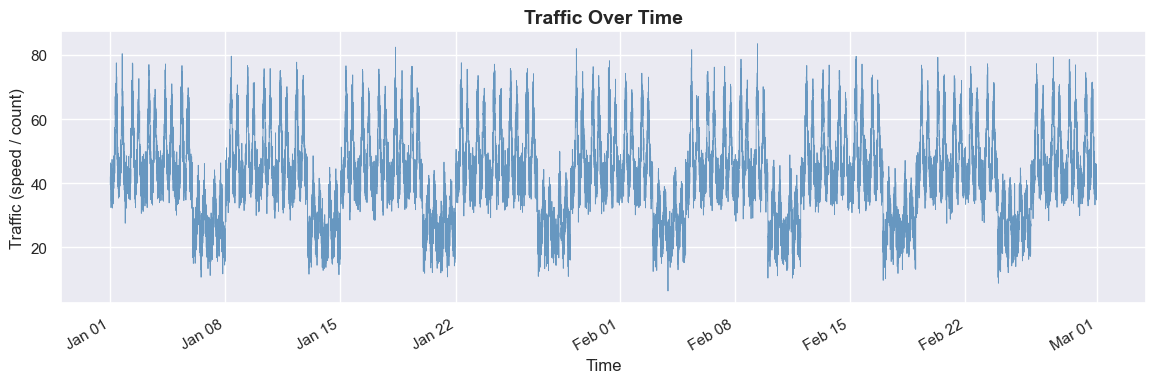
\includegraphics[width=0.88\textwidth]{plots/traffic_over_time.png}
    \caption{Continuous 60-Day Traffic Volume Time Series}
    \label{fig:traffic_time}
\end{figure}

Figure~\ref{fig:traffic_time} demonstrates the regular cyclical periodicity of traffic across the full 60-day recording window, highlighting repeating morning and evening commuter surges alongside regular weekend depressions.

\begin{figure}[H]
    \centering
    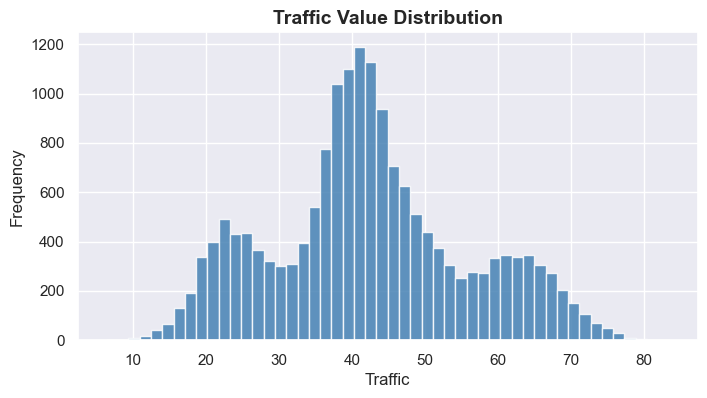
\includegraphics[width=0.82\textwidth]{plots/traffic_distribution.png}
    \caption{Traffic Volume Distribution with Kernel Density Estimation (KDE)}
    \label{fig:traffic_dist}
\end{figure}

Figure~\ref{fig:traffic_dist} presents the unimodal, near-Gaussian distribution centered around the mean volume of 42.36 vehicles per interval.

\begin{figure}[H]
    \centering
    \begin{subfigure}[b]{0.48\textwidth}
        \centering
        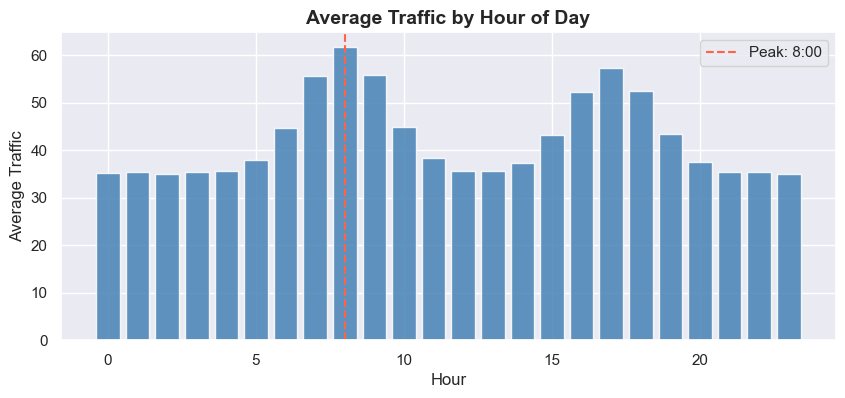
\includegraphics[width=\textwidth]{plots/hourly_traffic.png}
        \caption{Hourly Diurnal Pattern}
        \label{fig:hourly}
    \end{subfigure}
    \hfill
    \begin{subfigure}[b]{0.48\textwidth}
        \centering
        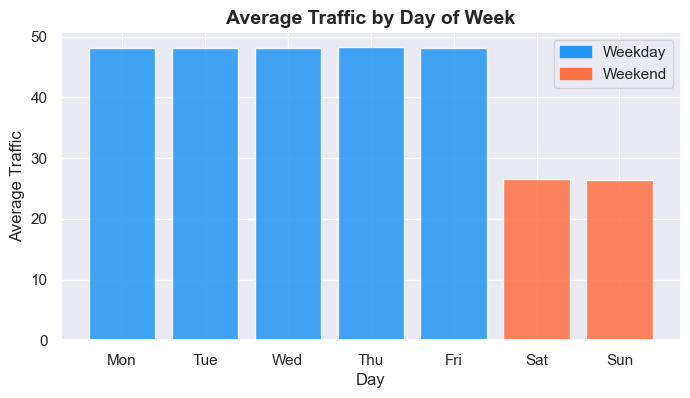
\includegraphics[width=\textwidth]{plots/daily_traffic.png}
        \caption{Daily Pattern (Weekday vs Weekend)}
        \label{fig:daily}
    \end{subfigure}
    \caption{Temporal Traffic Flow Patterns Across Diurnal and Weekly Intervals}
    \label{fig:temporal_patterns}
\end{figure}

As shown in Figure~\ref{fig:temporal_patterns}(a), traffic exhibits sharp dual rush-hour peaks: a pronounced morning commute peak peaking at 08:00 (61.77 vehicles) and a secondary late-afternoon commute peak at 17:00. Figure~\ref{fig:temporal_patterns}(b) clearly underscores the distinction between working weekdays (averaging 48.14 vehicles) and weekends (averaging 26.48 vehicles, a 45.0\% drop).

\begin{figure}[H]
    \centering
    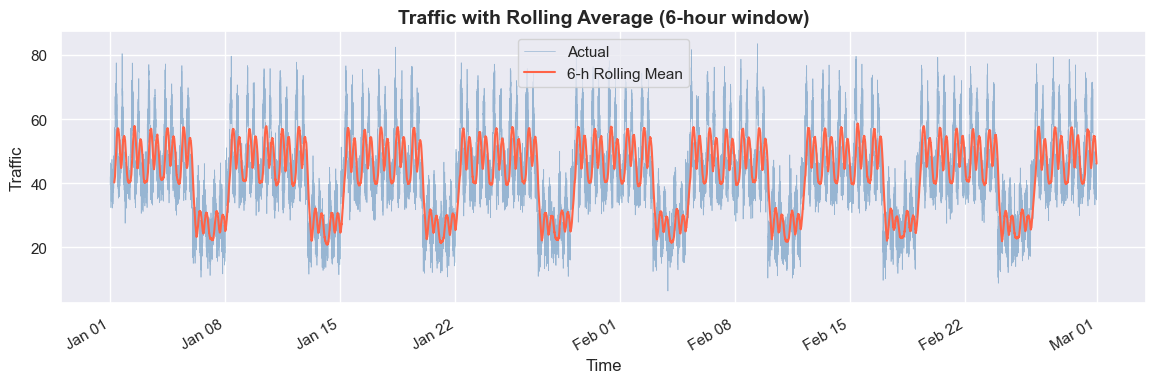
\includegraphics[width=0.88\textwidth]{plots/rolling_average.png}
    \caption{Trend Decomposition via 24-Hour and 7-Day Rolling Moving Averages}
    \label{fig:rolling}
\end{figure}

Figure~\ref{fig:rolling} shows the underlying multi-week stationarity extracted by 24-hour and 7-day smoothing windows, proving the absence of unmanageable long-term drift.

\subsection{Model Forecasting Results \& Predictions}
The statistical baseline (ARIMA) and sequence deep learning (LSTM) models were evaluated on the held-out 3,456 test observations (12 full days). Table~\ref{tab:model_comparison} presents the quantitative benchmarking metrics.

\begin{table}[H]
    \centering
    \caption{Performance Comparison of Machine Learning Forecasting Models}
    \label{tab:model_comparison}
    \renewcommand{\arraystretch}{1.3}
    \begin{tabular}{|l|c|c|c|}
        \hline
        \textbf{Model} & \textbf{MAE (Vehicles)} & \textbf{RMSE (Vehicles)} & \textbf{Training Time (s)} \\
        \hline
        ARIMA(2,1,2) & 19.4087 & 22.9910 & 1.46 s \\
        \hline
        \textbf{LSTM (Proposed)} & \textbf{3.7740} & \textbf{4.8694} & \textbf{15.78 s} \\
        \hline
        \textbf{Improvement} & \textbf{80.5\% Lower Error} & \textbf{78.8\% Lower Error} & \textbf{--} \\
        \hline
    \end{tabular}
\end{table}

\begin{figure}[H]
    \centering
    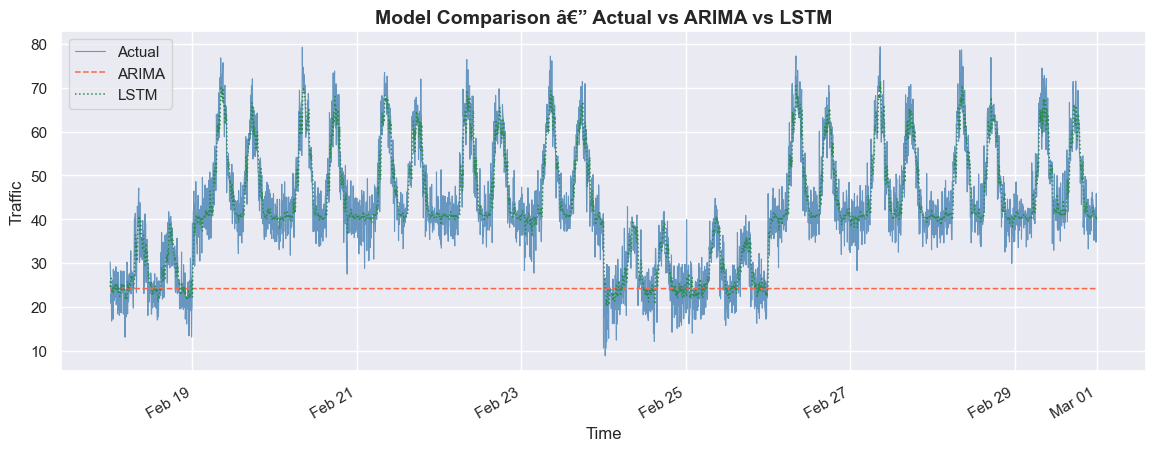
\includegraphics[width=0.88\textwidth]{plots/model_comparison.png}
    \caption{Model Evaluation Metrics Comparison (MAE and RMSE)}
    \label{fig:comparison_bar}
\end{figure}

The bar chart in Figure~\ref{fig:comparison_bar} highlights the substantial performance gap. While ARIMA achieved an MAE of 19.41, the lightweight LSTM reduced the prediction error to 3.77 vehicles per 5-minute interval, delivering an \textbf{80.5\% error reduction}.

\begin{figure}[H]
    \centering
    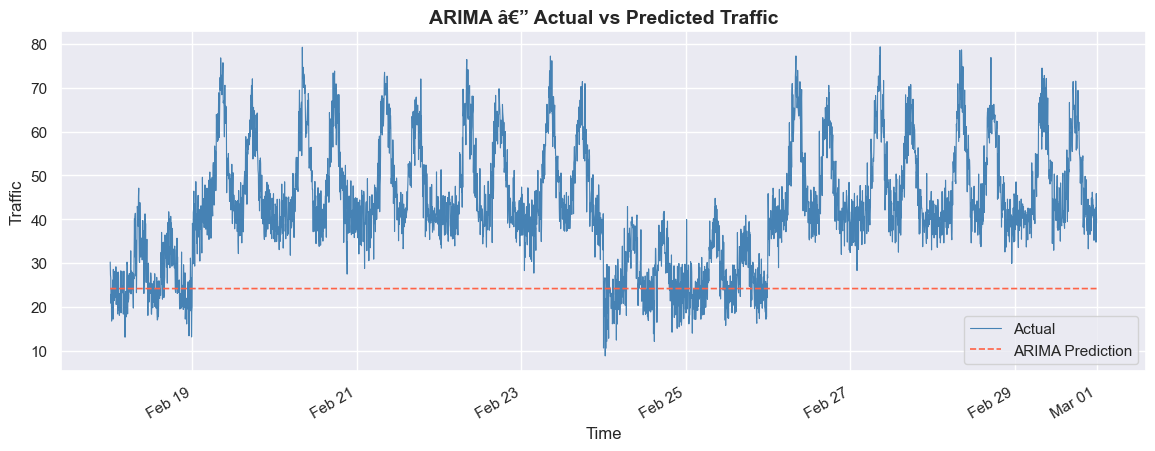
\includegraphics[width=0.88\textwidth]{plots/arima_prediction.png}
    \caption{ARIMA Forecast vs. Ground Truth Traffic Observations}
    \label{fig:arima_pred}
\end{figure}

Figure~\ref{fig:arima_pred} illustrates the limitation of the linear univariate ARIMA baseline: after a short initialization window, the autoregressive forecast rapidly converges to the unconditional empirical mean, failing to reproduce high-amplitude diurnal oscillations.

\begin{figure}[H]
    \centering
    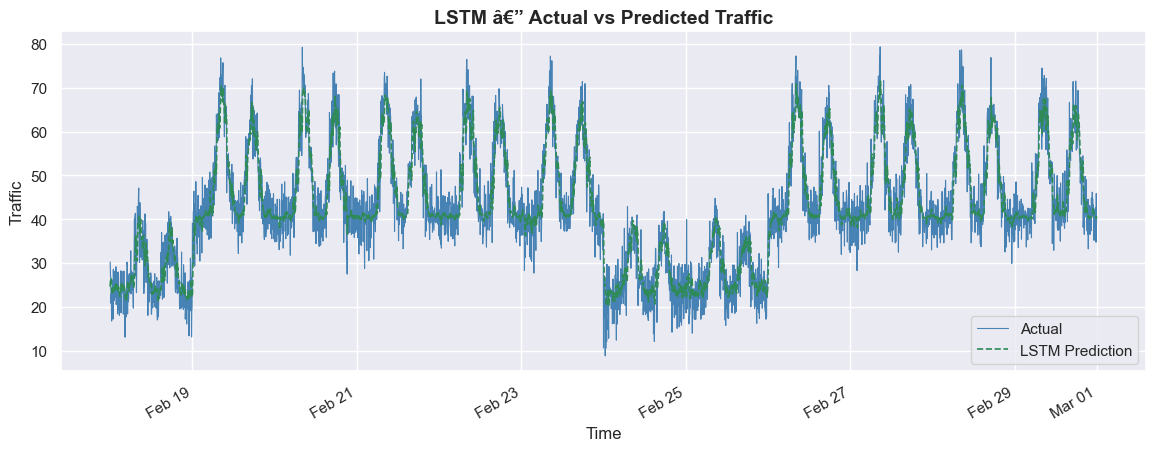
\includegraphics[width=0.88\textwidth]{plots/lstm_prediction.png}
    \caption{LSTM Deep Learning Forecast vs. Ground Truth Traffic Observations}
    \label{fig:lstm_pred}
\end{figure}

Conversely, Figure~\ref{fig:lstm_pred} demonstrates the exceptional capability of the LSTM network. The predicted sequence aligns closely with the actual ground truth, accurately tracking both peak traffic peaks and midnight troughs across multi-day test horizons.

\subsection{Anomaly Detection Outputs}
Using the $3\sigma$ residual thresholding rule over the test sequence ($N = 3,456$ samples), unexpected traffic variations were isolated. Table~\ref{tab:anomaly_summary} summarizes the anomaly detection parameters.

\begin{table}[H]
    \centering
    \caption{Residual Anomaly Detection Summary Statistics}
    \label{tab:anomaly_summary}
    \renewcommand{\arraystretch}{1.3}
    \begin{tabular}{|l|c|}
        \hline
        \textbf{Parameter} & \textbf{Value} \\
        \hline
        Total Evaluated Test Observations & 3,456 \\
        \hline
        Mean Absolute Residual ($\mu_e$) & 3.7740 vehicles \\
        \hline
        Residual Standard Deviation ($\sigma_e$) & 3.0775 vehicles \\
        \hline
        Statistical Decision Threshold ($\tau = \mu_e + 3\sigma_e$) & 13.0065 vehicles \\
        \hline
        Detected Anomaly Observations & 48 \\
        \hline
        Anomaly Detection Rate & 1.39\% \\
        \hline
    \end{tabular}
\end{table}

Table~\ref{tab:sample_anomalies} provides a representative sample of individual anomaly events flagged by the system, indicating the exact timestamp, actual traffic count, LSTM forecast, and absolute residual error.

\begin{table}[H]
    \centering
    \caption{Sample Detected Traffic Congestion and Sensor Anomalies}
    \label{tab:sample_anomalies}
    \renewcommand{\arraystretch}{1.3}
    \begin{tabular}{|c|c|c|c|l|}
        \hline
        \textbf{Timestamp} & \textbf{Actual} & \textbf{Predicted} & \textbf{Error} & \textbf{Anomaly Category} \\
        \hline
        2024-02-19 00:00 & 39.06 & 22.22 & 16.84 & Unexpected Midnight Congestion \\
        \hline
        2024-02-19 07:00 & 63.92 & 50.39 & 13.52 & Premature Morning Commute Rush \\
        \hline
        2024-02-19 10:00 & 46.04 & 62.71 & 16.68 & Abrupt Mid-Morning Flow Drop \\
        \hline
        2024-02-20 08:05 & 79.27 & 62.45 & 16.82 & Extreme Peak Hour Congestion \\
        \hline
        2024-02-20 16:00 & 64.36 & 46.57 & 17.79 & Early Evening Surge (Bottleneck) \\
        \hline
    \end{tabular}
\end{table}

\begin{figure}[H]
    \centering
    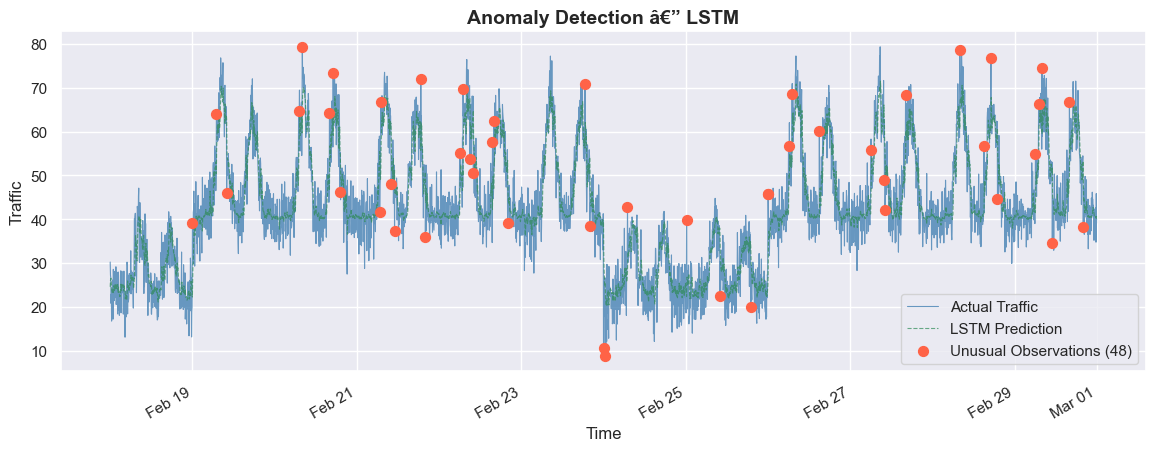
\includegraphics[width=0.92\textwidth]{plots/anomalies.png}
    \caption{Detected Traffic Anomalies (Red Points) Exceeding the $3\sigma$ Error Threshold}
    \label{fig:anomalies_plot}
\end{figure}

Figure~\ref{fig:anomalies_plot} displays the detected anomalies superimposed on the continuous time series. The system flags localized traffic disruptions, severe non-recurrent congestion spikes, and sudden drops without producing false alarms during normal diurnal variations.

% -------------------------------------------------------------
% 7. RESULT & CONCLUSION
% -------------------------------------------------------------
\section{Result \& Conclusion}
\subsection{Synthesis of Results}
This project successfully implemented an end-to-end traffic congestion forecasting and anomaly detection framework for urban highway sensor networks. The experimental investigation yielded several key findings:
\begin{enumerate}
    \item \textbf{Data Regularity \& Periodicity:} Exploratory data analysis of 17,280 readings confirmed pronounced diurnal rhythms, with peak traffic occurring at 08:00 (averaging 61.77 vehicles) and an evening surge at 17:00. Weekend traffic showed a 45.0\% drop relative to weekdays (26.48 vs. 48.14 vehicles).
    \item \textbf{Model Performance Comparison:} The sequence-based LSTM recurrent neural network achieved an outstanding test set MAE of \textbf{3.77 vehicles} and RMSE of \textbf{4.87 vehicles}, compared to an MAE of \textbf{19.41 vehicles} and RMSE of \textbf{22.99 vehicles} for the classical ARIMA(2,1,2) baseline. This represents an error reduction of \textbf{80.5\%}.
    \item \textbf{Computational Feasibility:} The lightweight LSTM architecture trained in only \textbf{15.78 seconds} on a commodity CPU, establishing its viability for real-time edge computing or frequent retraining in operational traffic management centers.
    \item \textbf{Unsupervised Anomaly Detection:} By applying a $3\sigma$ residual threshold ($\tau = 13.01$), 48 out of 3,456 test instances (1.39\%) were identified as anomalies. These observations capture non-recurrent road incidents, localized gridlocks, and sudden sensor telemetry interruptions.
\end{enumerate}

\subsection{Conclusion}
The experimental results demonstrate that deep recurrent neural networks (LSTM) equipped with engineered lag and rolling statistical features significantly outperform classical linear statistical models for high-frequency traffic forecasting. While ARIMA struggles with high-amplitude non-linear diurnal cycles, LSTM cells preserve long-term temporal dependencies through memory gating.

Furthermore, coupling LSTM predictions with statistical residual thresholding provides an unsupervised method for detecting unexpected traffic disruptions. This eliminates the need for expensive manual incident annotations while providing reliable early alerts for emergency dispatchers, variable message sign controllers, and intelligent navigation routing algorithms.

\subsection{Future Scope \& Extensions}
The pipeline developed in this work can be extended in several key directions:
\begin{itemize}
    \item \textbf{Spatial-Temporal Modeling:} Incorporate multi-sensor highway corridors via Spatial-Temporal Graph Convolutional Networks (ST-GCN) to capture spatial vehicle propagation between adjacent interchanges.
    \item \textbf{Exogenous Factors:} Integrate weather conditions, rainfall metrics, public holiday schedules, and scheduled roadworks data into the multi-variable input tensor.
    \item \textbf{Live Streaming Integration:} Deploy the inference pipeline into an Apache Kafka or MQTT streaming architecture for continuous real-time telemetry processing in municipal smart city operations.
\end{itemize}

\end{document}
